%!TEX root = ../these.tex

\chapter{%
  Основные формулы геометрии дуг на комплексной плоскости
}
\label{app:bulge}

Поскольку современное оборудование листовой фигурной резки с ЧПУ
использует для задания маршрута резки два геометрических примитива ---
отрезки прямых и дуги окружностей,
возникает вопрос удобного представления этих сущностей
для аналитического исследования и программной обработки.
Вооружившись тем фактом,
что дробно-линейное преобразование комплексной плоскости
переводит прямые в окружности и наоборот,
можно использовать единое представление обоих
геометрических примитивов,
к тому же значительно уменьшив обращение
к трансцендентным функциям.

Рассмотрим круговую дугу на рис.~\ref{fig:app.arc},
имея в виду,
что она может выражаться в отрезок прямой.
Зададим начальную точку $A$
и конечную точку $Z$,
а кривизну дуги выразим в виде параметра
$bulge$
по формуле:
\begin{equation}
  \beta = \tg \frac{\measuredangle ACZ}{4}
\end{equation}

\begin{figure}
  \centering
  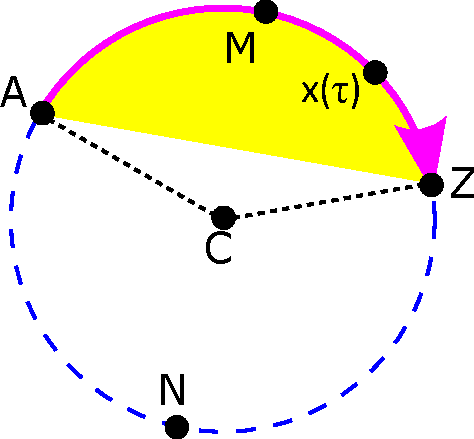
\includegraphics{arc.pdf}
  \caption{Основные элементы круговой дуги}
  \label{fig:app.arc}
\end{figure}

Знак параметра $\beta$
выберем положительным для дуг,
идущих против часовой стрелки
($\beta < 0$ на рис.~\ref{fig:app.arc} ).

Тогда легко подобрать формулу для положения
произвольной точки
$x(\tau)$ дуги,
параметризуемой положением
$\tau \in[-1,1]$:

\begin{equation}
  x(\tau) =
  \frac{A+Z}{2} + \frac{Z-A}{2}\frac{\tau - i \cdot \beta}{1 - i \cdot \beta \tau}
\end{equation}

Очевидно,
$x(-1) = A$,
$x(+1) = Z$.
